%\documentclass{sig-alternate-05-2015}
\documentclass[10pt,conference]{IEEEtran}
%\documentclass{llncs}
\usepackage{makeidx}
\usepackage{tabularx,colortbl}
\usepackage[dvipsnames]{xcolor}
\usepackage{flushend}
\usepackage{cite}
\usepackage{amsmath}
\usepackage{amsthm}
\usepackage{amssymb}
\usepackage{epsfig}
\usepackage{stmaryrd}
\usepackage{url}
\usepackage{multirow}
\usepackage{latexsym}
\usepackage{graphics}
\usepackage{graphicx}
\usepackage{enumitem}
\usepackage{comment}
\usepackage{longtable}
\usepackage{supertabular}
\usepackage{times}
\usepackage{listings}
\usepackage{subfigure}
\usepackage{color}
\usepackage{balance}
\usepackage{xspace}
\usepackage[ruled, vlined, linesnumbered]{algorithm2e}
\usepackage[autostyle]{csquotes}



%\theoremstyle{Definition}
%\newtheorem{definition}{Definition}
%%%
%\theoremstyle{Theorem}
%\newtheorem{theorem}{Theorem}


%\newcommand{\definition}{\noindent \textbf{Definition} \citation{}}
%\newcommand{\theorem}{\noindent \textbf{Theorem} \citation{}}
%\newcommand{\lemma}{\noindent \textbf{Lemma} \citation{}}

%\newdef{lemma}{Lemma}
%\newdef{definition}{Definition}
%\newdef{theorem}{Theorem}
%\newdef{corollary}{Corollary}
%\newdef{note}{Note}
%\newdef{axiom}{Axiom}

\newtheorem{theorem}{Theorem}
\newtheorem{definition}{Definition}

\newcommand{\mkeyword}[1]{\mbox{\texttt{#1}}}
\DeclareMathOperator{\kuop}{uop}
\DeclareMathOperator{\kbop}{bop}
\DeclareMathOperator{\kite}{ite}
\DeclareMathOperator{\kpre}{pre}
\DeclareMathOperator{\dom}{dom}
\DeclareMathOperator{\ktrue}{true}
\DeclareMathOperator{\kfalse}{false}
\DeclareMathOperator{\kselect}{select}
\DeclareMathOperator{\ran}{range}
\newcommand{\lbb}{[\![}
\newcommand{\rbb}{]\!]}
\newcommand{\expr}{\phi}
\newcommand{\exprS}{\Phi}
\newcommand{\mike}[1]{\textcolor{red}{#1}}
\newcommand{\janet}[1]{\textcolor{blue}{#1}}
\newcommand{\darren}[1]{\textcolor{green}{#1}}
\newcommand{\danielle}[1]{\textcolor{orange}{#1}}

\sloppypar



\begin{document}

\definecolor{gold}{rgb}{0.90,.66,0}
\definecolor{dgreen}{rgb}{0,0.6,0}
\newcommand{\stateequiv}{\equiv_{s}}
\newcommand{\traceequiv}{\equiv_{\sigma}}
\newcommand{\ta}{\text{TA}}
\newcommand{\cta}{\text{TA$_{C}$}}
\newcommand{\tta}{\text{TA$_{T}$}}
\newcommand{\ucalg}{\texttt{\small{IVC\_UC}}}
\newcommand{\ucbfalg}{\texttt{\small{IVC\_UCBF}}}
\newcommand\doesnotentail{\mkern-2mu\not\mkern2mu\vdash}


\title{ICSE paper outline}
%


\author{\IEEEauthorblockN{Danielle Stewart\IEEEauthorrefmark{1}, Jing (Janet) Liu\IEEEauthorrefmark{2}, Michael W. Whalen\IEEEauthorrefmark{1}, Darren Cofer\IEEEauthorrefmark{2}, Mats Heimdahl\IEEEauthorrefmark{1}, Michael Peterson\IEEEauthorrefmark{3}}
\IEEEauthorblockA{\IEEEauthorrefmark{1}University of Minnesota\\Department of Computer
	Science and Engineering\\Email: \{dkstewar, whalen, heimdahl\}@umn.edu}
\IEEEauthorblockA{\IEEEauthorrefmark{2}Rockwell Collins\\
	Advanced Technology Center\\Email: \{Jing.Liu, Darren.Cofer\}@rockwellcollins.com}
\IEEEauthorblockA{\IEEEauthorrefmark{3}Rockwell Collins\\
	Commercial Systems Flight Controls Safety Engineering\\Email: Michael.Peterson@rockwellcollins.com}}


\maketitle

\begin{abstract}
Risk and fault analysis are important activities that help to ensure that critical systems operate in an expected way. As critical systems become more dependent on software components, analysis regarding fault propagation through these software components becomes more important. The methods used to perform these analyses require understandability from the side of the analyst, scalability in terms of system size, and mathematical correctness in order to be sufficient proof that a system is safe. Determination of the events that can cause failures to propagate through a system as well as the affects of these propagations can be a time consuming and error prone process. In this paper, we describe a technique for determining these events with the use of a model checker and producing safety analysis artifacts that encode pertinant system safety information. We describe the technique of generating these safety artifacts, prove that our approach is sound, and describe its implementation in the Osate tool suite for AADL. We then present experiments in which we benchmark our approach in terms of scalability and the artifacts produced. 
\end{abstract}

\section{Introduction}
\label{sec:intro}

%This paper describes a new methodology with tool support for model based safety analysis. It is implemented as a {\em Safety Annex} for the Architecture Analysis and Design Language (AADL). The Safety Annex provides the ability to describe faults and faulty component behaviors in AADL models. In contrast to previous AADL-based approaches, the Safety Annex leverages a formal description of the nominal system behavior to propagate faults in the system. This approach ensures consistency with the rest of the system development process and simplifies the work of safety engineers. The language for describing faults is extensible and allows safety engineers to weave various types of faults into the nominal system model. The Safety Annex supports the injection of faults into component level outputs, and the resulting behavior of the system can be analyzed using model checking through the Assume-Guarantee Reasoning Environment (AGREE).

System safety analysis techniques are well-established and are a required activity in the development of safety-critical systems. Model-based systems engineering (MBSE) methods and tools based on formal methods now permit system-level requirements to be specified and analyzed early in the development process~\cite{NFM2012:CoGaMiWhLaLu,CAV2015:BoCiGrMa}. While model-based development methods are widely used in the aerospace industry, they are only recently being applied to system safety analysis.  

%How can we leverage these model-based methods and tools to perform safety analysis based on models of the system architecture and initial functional decomposition? Can these design models be integrated into the safety analysis process to help guarantee accurate and consistent results?
%Seeking solutions to these questions are especially important as the amount of safety-critical hardware and software in various domains has drastically increased due to the demand for greater autonomy, capability, and connectedness.

In this paper, we describe a {\em Safety Annex} for the Architecture Analysis and Design Language (AADL)~\cite{FeilerModelBasedEngineering2012} that provides the ability to reason about faults and faulty component behaviors in AADL models. In the Safety Annex approach, we use formal assume-guarantee contracts to define the nominal behavior of system components. The nominal model is then verified using the Assume Guarantee Reasoning Environment (AGREE)~\cite{NFM2012:CoGaMiWhLaLu}. The Safety Annex  provides a way to weave faults into the nominal system model and analyze the behavior of the system in the presence of faults. The Safety Annex also provides a library of common fault node definitions that is customizable to the needs of system and safety engineers. Our approach adapts the work of Joshi et. al in
~\cite{Joshi05:Dasc} to the AADL modeling language, and provides a domain specific language for the kinds of analysis performed manually in previous work~\cite{Stewart17:IMBSA}.  %More information on the approach is available in~\cite{Stewart17:IMBSA}, and the tool and relevant documentation can be found at: \small \url{https://github.com/loonwerks/AMASE/}. \normalsize

There are other tools purpose-built for safety analysis, including AltaRica~\cite{PROSVIRNOVA2013127}, smartIFlow~\cite{info8010007} and xSAP~\cite{DBLP:conf/tacas/BittnerBCCGGMMZ16}. These notations are separate from the system development model. Other tools extend existing system models, such as HiP-HOPS~\cite{CHEN201391} and the AADL Error Model Annex, Version 2 (EMV2)~\cite{EMV2}. EMV2 uses enumeration of faults in each component and explicit propagation of faulty behavior to perform safety analysis. The required propagation relationships must be manually added to the system model and can become complex, leading to potential omissions and inconsistencies.

In contrast, the Safety Annex supports model checking and quantitative reasoning by attaching behavioral faults to components and then using the normal behavioral propagation and proof mechanisms built into the AGREE AADL annex. This allows users to reason about the evolution of faults over time, and produce counterexamples demonstrating how component faults lead to system failures. It can serve as the shared model to capture system design and safety-relevant information, and produce both qualitative and quantitative description of the causal relationship between faults/failures and system safety requirements.
%
Thus, the contributions of the Safety Annex and this paper are:
\begin{itemize}
\item Close integration of behavioral fault analysis into an {\em architectural design language} AADL, which allows close connection between system and safety analysis and system generation from the model (unlike AltaRica, smartIFlow, and xSAP),
\item support for {\em behavioral specification of faults} and their {\em implicit propagation} through behavioral relationships in the model, in contrast to existing AADL-based annexes (HiP-HOPS and EMV2),
\item additional support for {\em explicit} propagation of faults to capture binding relationships between hardware and software and logical and physical communications beyond what is supported in xSAP, and
\item guidance on integration into a traditional safety analysis process.
\end{itemize}
%\mike{What are our contributions?}


\section{Background}
This section provides a high level description of the pieces of the puzzle necessary in order to understand our approach. We describe the relevant algorithms and tools in order to make the later formalisms fit into the full picture. 

\subsection{Inductive Validity Cores}

Given a complex model, it is often useful to extract traceability information related to the proof, in other words, which portions of the model were necessary to construct the proof. An algorithm was introduced by Ghassabani, et. al. to provide Inductive Validity Cores (IVCs) as a way to determine which model elements are necessary for the inductive proofs of the safety properties for sequential systems~\cite{GhassabaniGW16}. Given a safety property of the system, a model checker can be invoked in order to construct a proof of the property. The IVC generation algorithm can extract traceability information from that proof process and return the model elements required in order to prove the property. A short time later, this algorithm was refined in order to produce the minimal set of such IVC elements~\cite{Ghassabani2017EfficientGO}. 

This algorithm is of interest to us for the following reason. By letting the negation of the safety property of interest be our top level event, we can utilize the algorithm to find the set of minimal IVCs which will tell us the minimal model elements (including faults) necessary to prove that this top level event occurs. In other words, we will know the minimal set of events required in order to cause the occurance of the top level event. These model elements consist of the active faults present in the system and the contracts of components that were effected by the presence of the fault. This gives a trace of how the fault propagates through system components and how the software behaves in the presence of the faults. 

In section III, we show the formal definitions of IVCs in detail. \\

Our approach utilizes a few tools in order to generate the artifacts of interest and a brief background will be helpful. and hence the rest of the background section consists of a brief description of AADL, AGREE, and the SOTERIA tools and languages. 

\subsection{Architecture Analysis and Design Language}
We are using the Architectural Analysis and Design Language (AADL)~\cite{FeilerModelBasedEngineering2012} to construct system architecture models.  AADL is an SAE International standard that defines a language and provides a unifying framework for describing the system architecture for ``performance-critical, embedded, real-time systems''~\cite{AADL_Standard}. From its conception, AADL has been designed for the design and construction of avionics systems.  Rather than being merely descriptive, AADL models can be made specific enough to support system-level code generation.  Thus, results from analyses conducted, including the new safety analysis proposed here, correspond to the system that will be built from the model.  

An AADL model describes a system in terms of a hierarchy of components and their interconnections, where each component can either represent a logical entity (e.g., application software functions, data) or a physical entity (e.g., buses, processors). An AADL model can be extended with language annexes to provide a richer set of modeling elements for various system design and analysis needs (e.g., performance-related characteristics, configuration settings, dynamic behaviors). The language definition is sufficiently rigorous to support formal analysis tools that allow for early phase error/fault detection.

\subsection{Compositional Analysis} Compositional analysis of systems was introduced in order to address the scalability of model checking large software systems. Monolithic verification and compositional verification are two ways that mathematical verification of component properties can be performed. In monolithic analysis, the model is flattened and the top level properties are proved using only the leaf level contracts of the components. On the other hand, the analysis can be performed compositionally following the architecture hierarchy such that analysis at a higher level is based on the components at the next lower level.  When compared to monolithic analysis (i.e., analysis of the flattened model composed of all components), the compositional approach allows the analysis to scale to much larger systems~\cite{NFM2012:CoGaMiWhLaLu}. 

\subsection{Assume Guarantee Reasoning Environment}
The Assume Guarantee Reasoning Environment (AGREE) is a tool for formal analysis of behaviors in AADL models~\cite{NFM2012:CoGaMiWhLaLu}.  It is implemented as an AADL annex and annotates AADL components with formal behavioral contracts. Each component's contracts can include assumptions and guarantees about the component's inputs and outputs respectively, as well as predicates describing how the state of the component evolves over time.

AGREE translates an AADL model and the behavioral contracts into Lustre~\cite{Halbwachs91:IEEE} and then queries a user-selected
model checker to conduct the back-end analysis. The analysis can be performed compositionally following the architecture hierarchy such that analysis at a higher level is based on the components at the next lower level.  When compared to monolithic analysis (i.e., analysis of the flattened model composed of all components), the compositional approach allows the analysis to scale to much larger systems~\cite{QFCS15:backes}. 

\subsection{Safety Annex for AADL}
The Safety Annex for AADL is a tool that provides the ability to reason about faults and faulty component behaviors in AADL models~\cite{Stewart17:IMBSA,SATechReport}. In the Safety Annex approach, formal assume-guarantee contracts are used to define the nominal behavior of system components. The nominal model is verified using AGREE. The Safety Annex weaves faults into the nominal model and analyzes the behavior of the system in the presence of faults. The tool supports behavioral specification of faults and their implicit propagation through behavioral relationships in the model as well as provides support to capture binding relationships between hardware and software compönents of the system. 

\subsection{SOTERIA}
The Safe and Optimal Techniques Enabling Recovery, Integrity, and Assurance (SOTERIA) tool is used to perform safety analysis of Integrated Modular Avionics (IMA) systems~\cite{SOTERIAproject}. In the SOTERIA project, a compositional modeling language was developed and this language is used as input in order to automatically synthesize the qualitative and quantitative safety analyses. The tool is compositional in that it requires safety aspects at each component level which enables the generation of compositional fault trees. 

\begin{figure}[h]
\begin{center}
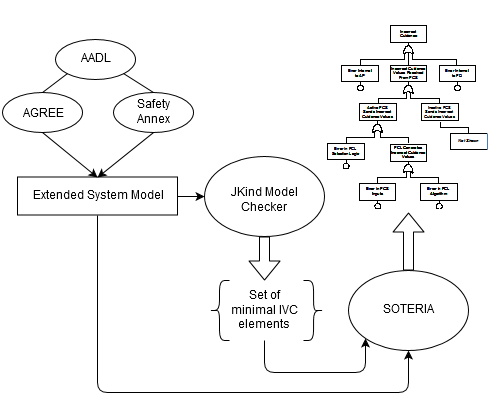
\includegraphics[width=8cm]{images/processFTA.png}
\caption{Outline of the fault tree generation process} \label{fig:processFTA}
\end{center}
\end{figure}

\subsection{Fault Tree Analysis} A Fault Tree (FT) is a directed acyclic graph whose leaves model component failures and whose gates model failure propagation. The system failure under examination is the root of the tree and is called the Top Level Event (TLE). The Basic Events (BE) are the events that can occur in the system which lead to the TLE and in the graphical model, these correspond to the leaves. Figure~\ref{fig:introFT} shows a simple example of a fault tree based on SAE ARP4761~\cite{SAE:ARP4761}. In this example, the top level event corresponds to an aircraft losing all wheel braking. In order for this event to occur, all of the basic events must occur. This is seen through the use of the AND gate below the top level event. The gates in the fault tree describe how failures propagate through the system. Each gate has one output and one or more inputs. In Figure~\ref{fig:introFT}, the AND gate has three inputs and one output. The leaves of the tree represent the basic events of the system and in the case of this fault tree, these three events are also the \textit{minimum cut set} for this top level event. The minimal cut set is the minimum set of basic events that must occur together in order to cause the TLE to occur. Finding these sets is important to FTA and has been an active area of interest in the research community since fault trees were first described in Bell Labs in 1961~\cite{historyFTA}. 

\begin{figure}[h]
\begin{center}
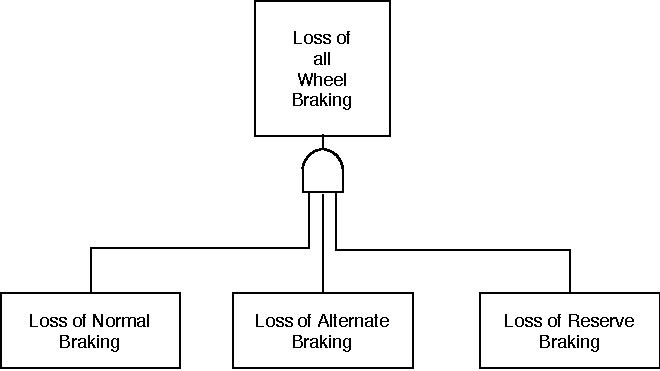
\includegraphics[width=8cm]{images/introFT2.pdf}
\caption{A simple fault tree} \label{fig:introFT}
\end{center}
\end{figure}

There are two main types of FTA that we differentiate here as \textit{qualitative} analysis and \textit{quantitative} analysis. In qualitative analysis, the structure of the fault tree is considered and the cut sets are a way to indicate which combinations of component failures will cause the system to fail. On the other hand, in quantitative analysis the probability of the TLE is calculated given the probability of occurance of the basic events. 

The formal definition of a fault tree is provided in section III and more details regarding quantitative and qualitative FTA is explained there as well. 

The general outline of our process is as follows and is shown in Figure~\ref{fig:processFTA} (Note: the fault tree shown in Figure~\ref{fig:processFTA} is generic and the text is irrelevant). The AADL system model is annotated with behavioral contracts using AGREE and then extended with faults using the Safety Annex. These three things together make the extended system model as shown in the figure. The extended system model is given to the JKind model checker~\cite{2017arXiv171201222G} which outputs the minimal sets of IVC elements for each layer of the architecture. These IVC elements and pertinant details of the extended system model is given to the SOTERIA tool whose output is the graphical fault tree representation of the input. 


\section{Methodology}
Given a complex model, it is often useful to extract traceability information related to the proof, in other words, which portions of the model were necessary to construct the proof. To this end, an algorithm was developed that efficiently computes the \textit{inductive validity cores} (IVC) within a model necessary for the proofs of safety properties for sequential systems \cite{DBLP:journals/corr/GhassabaniGW16}. 

\subsection{Preliminaries}
Given a state space $S$, a transition system $(I,T)$ consists of the initial state predicate $I : S \rightarrow \{0,1\}$ and a transition step predicate $T : S \times S \rightarrow \{0,1\}$. Reachability for $(I,T)$ is defined as the smallest predicate $R : S \rightarrow \{0,1\}$ which satisfies the following formulas:
\begin{center}
$\forall s. I(s) \Rightarrow R(s)$\\
$\forall s, s' .  R \land T(s,s') \Rightarrow R(s')$\\
\end{center}
A safety property $\mathcal{P} : S \to \{0,1\}$ is a state predicate. A safety property $\mathcal{P}$ holds on a transition system $(I,T)$ if it holds on all reachable states. More formally, $\forall s . R(s) \Rightarrow \mathcal{P}(s)$. When this is the case, we write $(I,T) \vdash\mathcal{P}$. Following Ghassabani, et. al. \cite{DBLP:journals/corr/GhassabaniGW16}, we formalize IVCs as follows.\\

\begin{definition}Inductive Validity Core\\
 Let $(I,T)$ be a transition system and let $\mathcal{P}$ be a safety property with $(I,T) \vdash \mathcal{P}$. Then $S \subseteq T$ is an \textit{inductive validity core} for $(I,T) \vdash \mathcal{P}$ iff $(I,S) \vdash\mathcal{P}$.  \\
\end{definition}

\begin{definition}Minimal Inductive Validity Core\\
An inductive validity core $S$ for $(I,T) \vdash \mathcal{P}$ is minimal iff $! \exists S' . S' \subset S \ni (I,S') \vdash \mathcal{P}$. \\
\end{definition}

A fault tree is a directed acyclic graph (DAG) consisting of the node types \textit{events} and \textit{gates}. An event is an occurance within the system, typically the failure of a subsystem down to an individual component. Events can be grouped into \textit{basic events} (BEs), which occur independently, and \textit{intermediate events} which occur dependently and are caused by one or more other events. The event at the top of the tree, the \textit{top level event} (TLE), is the event being analyzed. This event models the failure of the system (or subsystem) under consideration. The gates represent how failures propagate through the system and how failures in subsystems can cause system wide failures. The two main logic symbols used are the Boolean logic AND-gates and OR-gates.
An AND-gate is used when the undesired top level event can only occur when all the lower conditions are true. The OR-gate is used when the undesired event can occur if any one or more of the next lower conditions is true. This is not a comprehensive list of gate types, but we focus our attention on these two common gate types.\\

To formalize a fault tree (FT), we use $GateTypes = \{And, Or\}$. Following Ruijters, et. al. \cite{RuijtersSurvey}, we formalize FT as follows. \\

\begin{definition}Fault Tree\\ 
A FT is a 4-tuple $F = \langle BE, G, T, I \rangle$ consisting of the following components. 
\begin{itemize}
\item BE is the set of basic events
\item G is the set of gates with $BE \cap G = \emptyset$. We write $E = BE \cup G$ for the set of elements.
\item $T: G \to GateTypes$ is a function that describes the type of each gate.
\item $I: G \to P(E)$ describes the inputs of each gate. We require that $I(G) \neq \emptyset$.
\end{itemize}
\end{definition}

The graph formed by $\langle E, I \rangle$ is a directed acyclic graph with a unique root $TLE$ which is reachable from all nodes. \\

\begin{definition}Semantics of a Fault Tree\\  
The semantics of FT F is a function $\pi_F : \mathcal{P}(BE) \times E \vdash \{0,1\}$ where $\pi_F(S, e)$ indicates whether $e$ fails given the set $S$ of failed BEs. It is defined as follows. 
\begin{itemize}
\item For $e \in BE$, $\pi_F(S,e) = e \in S$.
\item For $g \in G$ and $T(g) = And$, let\\ $\pi_F(S,g) = \land_{x \in I(g)} \pi_F(S, x)$
\item For $g \in G$ and $T(g) = Or$, let\\ $\pi_F(S,g) = \lor_{x \in I(g)} \pi_F(S, x)$ \\
\end{itemize}
\end{definition}

The interpretation of the TLE $t$ is written as $\pi_F(S,t) = \pi_F(S)$. If the failure of $S$ causes the TLE to occur, we write $\pi_F(S) = 1$. 

 In qualitative analysis, cut sets and minimal cut sets provide information about the vulnerabilities of a system in terms of its basic events. A \textit{cut set} is a set of components that together can cause a system to fail. A \textit{minimal cut set} is a cut set which contains the minimum number of basic events required in order to cause the TLE to occur. More formally, these are defined as follows. \\

\begin{definition}Cut Set\\   
 $C \subseteq BE$ is a cut set of FT F if $\pi_F(C) = 1$. \\
\end{definition}

\begin{definition}Minimal Cut Set\\    
$C \subseteq BE$ is a MCS if $\pi_F(C) = 1 \land \forall C' \subset C. \pi_F(C') = 0$. In other words, a minimal cut set (MCS) is a cut set of which no subset is a cut set. \\
\end{definition}

Given the formalisms defined previously, we show that finding the minimal IVCs is equivalent to finding the MCS. \\

\begin{theorem} Finding all minimal IVCs is equivalent to finding the set of all MCSs\\

\begin{proof} 
Let $T = \{f_1, f_2, ..., f_n\}$ be the set of model elements corresponding to faults for the components and let $\mathcal{P}_{tle}$ be the top level event (TLE). By the definition for IVC, we know that $S \subseteq T$ is an IVC for $(I, T) \vdash \mathcal{P}_{tle}$ iff $(I, S) \vdash \mathcal{P}_{tle}$. 
In this case, $\pi_F(S) = 1$, i.e. given the set $S \subseteq T$ of failed model elements, the top level event occurs. 
Since $S$ is minimal IVC, for any $M \subset S$, $(I, M) \doesnotentail \mathcal{P}_{tle}$. Hence it follows that $\pi_F(M) = 0$ for any $M \subset S$.
\end{proof}
\end{theorem}

\subsection{Quantitative analysis}
Quantitative analysis methods derive numerical values for fault trees. One of these calculations that is of particular interest to the safety engineering community is the probability of the occurance of the top level event (TLE). This value is of interest because in certain critical systems, the top level properties must be proved safe within a certain probabilistic threshold~\cite{SAE:ARP4761}. The next section describes probability theory and provides a description of how they are used to calculate the probability of the TLE. These definitions are based on the ones given in~\cite{RuijtersSurvey}.\\

\danielle{I will add the probability formalisms here later. For now, I just want to clarify my findings regarding the proof that Mike was talking about yesterday.}\\
Assume events occur independently. \\

Or gate: \\
Probability is defined as follows: \\
$P(A \lor B) = P(A) + P(B) - P(A \land B)$. \\
Assume that the probability of events A, B is quite small (this is called the Rare Event Approximation). Then the term $P(A \land B)$ will also be quite small and hence is an ``error term". If we drop this term from the calculations, we end up with the approximated probability being: $P(A) + P(B) \geq P(A) + P(B) - P(A \land B)$. \\ This is clearly a conservative estimate. \danielle{It is also shown in the Fault Tree Handbook that this error is less than 0.1 I believe. I will have to review that again, but there is a bound on this error that has been previously proven.}

And gate: \\
With the calculations of the and gate, this is where independence is really required. Using Bayes Rule, we have $P(A \land B) = P(B)P(A|B) = P(A)P(B|A)$ for conditionally dependent events and $P(A \land B) = P(B)P(A)$ for independent events. If we assume independence when the events are NOT independent, in the worst case scenario, we get something like $B$ is completely dependent on $A$. Therefore $P(B|A) = 1$ and $P(A \land B) = P(B) \geq P(B)P(A)$. Not a conservative estimation. In the case of dependence, joint probability values would be required (acommon cause analysis).  \\

\danielle{Any other kind of gate uses combinations of these rules. These are not proofs that I made, I just looked at the logic of the operations. I am not sure how much we want to include in the paper. I assume a description is necessary, but a proof? No, this isn't a proof... This is just following definitions down a short little jaunt in the woods.}








\section{Case Studies}

To demonstrate the effectiveness of this approach and compare to state of the art existing tools, we describe two case studies.

\subsection{Wheel Brake System}
The Wheel Brake System (WBS) described in AIR6110~\cite{AIR6110} is a well-known example that has been used as a case study for safety analysis, formal verification, and contract based design~\cite{DBLP:conf/cav/BozzanoCPJKPRT15, 10.1007/978-3-319-11936-6-7, CAV2015:BoCiGrMa, Joshi05:SafeComp}. The preliminary work for the safety annex used a simplified model of the WBS~\cite{Stewart17:IMBSA}. In order to demonstrate scalability of our tools and compare results with other studies, we constructed a functionally and structurally equivalent AADL version of one of the most complex WBS NuSMV/xSAP models (arch4wbs) described in~\cite{DBLP:conf/cav/BozzanoCPJKPRT15}. We refer readers to this publication for diagrams of the full arch4wbs model~\cite{DBLP:conf/cav/BozzanoCPJKPRT15}. A simplified diagram taken from ARP4761 is shown in Figure~\ref{fig:wbs_arp4761}. 

\begin{figure}[h]
\begin{center}
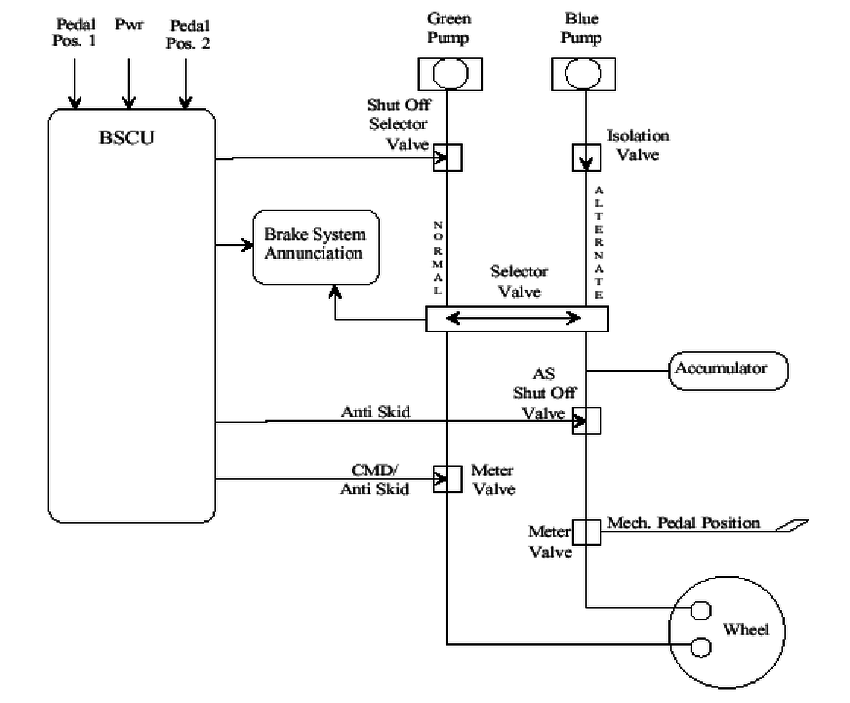
\includegraphics[width=8cm]{images/wbs_arp4761}
\caption{Simplified model of the WBS from ARP4761} \label{fig:wbs_arp4761}
\end{center}
\end{figure}

\subsubsection{WBS architecture description}
The WBS is composed of two main parts: the control system and the physical system. The control system electronically controls the physical system and contains a redundant Braking System Control Unit (BSCU) in case of failure. The physical system consists of the hydraulic circuits running from hydraulic pumps to wheel brakes. This is what provides braking force to each of the 8 wheels of the aircraft.

There are three operating modes in the WBS model. In \textit{normal} mode, the system uses the \textit{green} hydraulic circuit. The normal system is composed of the green hydraulic pump and one meter valve per each of the 8 wheels (shown as one wheel in Figure~\ref{fig:wbs_arp4761}). Each of the 8 meter valves are controlled through electronic commands coming from the BSCU. These signals provide brake commands as well as antiskid commands for each of the wheels. The braking command is determined through a sensor on the pilot pedal position. The antiskid command is calculated based on information regarding ground speed, wheel rolling status, and braking commands.

In \textit{alternate} mode, the system uses the \textit{blue} hydraulic circuit.  The wheels are all mechanically braked in pairs (one pair per landing gear). The alternate system is composed of the blue hydraulic pump, four meter valves, and four antiskid shutoff valves. The meter valves are mechanically commanded through the pilot pedal corresponding to each landing gear. If the system detects lack of pressure in the green circuit, the selector valve switches to the blue circuit. This can occur if there is a lack of pressure from the green hydraulic pump, if the green hydraulic pump circuit fails, or if pressure is cut off by a shutoff valve. If the BSCU channel becomes invalid, the shutoff valve is closed.

The last mode of operation of the WBS is the \textit{emergency} mode. This is supported by the blue circuit but operates if the blue hydraulic pump fails. The accumulator pump has a reserve of pressurized hydraulic fluid and will supply this to the blue circuit in emergency mode.

The model contains 30 different kinds of components, 169 component instances, a model depth of 5 hierarchical levels.  The model includes one top-level assumption and  11 top-level system properties, with 113 guarantees allocated to subsystems.  There are a total of 33 different fault types and 141 fault instances within the model.  The large number of fault instances is due to the redundancy in the system design and its replication to control 8 wheels. An example property is to ensure no inadvertent braking of each of the 8 wheels.  This means that if all power and hydraulic pressure is supplied (i.e., braking is commanded), then either the aircraft is stopped (ground speed is zero), or the mechanical pedal is pressed, or brake force is zero, or the wheel is not rolling.



\section{Related Work}
\label{sec:related_work}

A model-based approach for safety analysis was proposed by Joshi et. al in \cite{Joshi05:Dasc, Joshi05:SafeComp, Joshi07:Hase}.  In this approach, a safety analysis system model (SASM) is the central artifact in the safety analysis process, and traditional safety analysis artifacts, such as fault trees, are automatically generated by tools that analyze the SASM.

The contents and structure of the SASM differ significantly across different conceptions of MBSA.  We can draw distinctions between approaches along several different axes.  The first is whether they propagate faults explicitly through user-defined propagations, which we call {\em failure logic modeling} (FLM) or through existing behavioral modeling, which we call {\em failure effect modeling} (FEM).  The next is whether models and notations are {\em purpose-built} for safety analysis vs. those that extend {\em existing system models} (ESM).

For FEM approaches, there are several additional dimensions.  One dimension involves whether {\em causal} or {\em non-causal} models are allowed.  Non-causal models allow simultaneous (in time) bi-directional %failure
error propagations, which allow more natural expression of some failure types (e.g. reverse flow within segments of a pipe), but are more difficult to analyze.  A final dimension involves whether analysis is {\em compositional} across layers of hierarchically-composed systems or {\em monolithic}.  Our approach is an extension of AADL (ESM), causal, compositional, mixed FLM/FEM approach.

%We believe this is in a unique area of the trade space compared to other state-of-the-art MBSA approaches.

%Formal model based systems engineering (MBSE) methods and tools now permit system level requirements to be specified and analyzed early in the development process~\cite{QFCS15:backes,CIMATTI2015333, NFM2012:CoGaMiWhLaLu, hilt2013:MuWhRaHe}. Design models from which aircraft systems are developed can be integrated into the safety analysis process to help guarantee accurate and consistent results. Integration of MBSA into safety analysis process is described by Bozzano and Villafiorita~\cite{Bozzano:2010:DSA:1951720}. There are tools that currently support reasoning about faults in architecture description languages such as SysML and AADL. We provide here a brief overview of the most relevant safety analysis tools.

%In analyzing an EMV2 model of the WBS, we found missing feedback loops between the wheels and BSCU
%Interactions are easily overlooked by analysts and thus not explicitly described. In our approach, faults are injected into the system and behaviorally propagated through the use of assume-guarantee statements in AGREE. This avoids the difficulties inherent with explicit fault enumeration and propagation.

Tools such as the AADL Error Model Annex, Version 2 (EMV2)~\cite{EMV2} and HiP-HOPS for EAST-ADL~\cite{CHEN201391} are {\em FLM}-based {\em ESM} approaches.  As previously discussed, given many possible faults, these propagation relationships require substantial user effort and become more complex.  In addition, it becomes the analyst's responsibility to determine whether faults can propagate; missing propagations lead to unsound analyses.  In our Safety Annex, propagations occur through system behaviors (defined by the nominal contracts) with no additional user effort.

Closely related to our work is the model-based safety assessment toolset called COMPASS (Correctness, Modeling project and Performance of Aerospace Systems)~\cite{10.1007/978-3-642-04468-7_15}.  COMPASS is a mixed {\em FLM/FEM}-based, {\em causal} {\em compositional} tool suite that uses the SLIM language, which is based on a subset of AADL, for its input models~\cite{5185388, criticalembeddedsystems}. In SLIM, a nominal system model and the error model are developed separately and then transformed into an extended system model.  This extended model is automatically translated into input models for the NuSMV model checker~\cite{Cimatti2000, NuSMV}, MRMC (Markov Reward Model Checker)~\cite{Katoen:2005:MRM:1114692.1115230, MRMC}, and RAT (Requirements Analysis Tool)~\cite{RAT}. The safety analysis tool xSAP~\cite{DBLP:conf/tacas/BittnerBCCGGMMZ16} can be invoked in order to generate safety analysis artifacts such as fault trees and FMEA tables~\cite{compass30toolset}.  COMPASS is an impressive tool suite, but some of the features that make AADL suitable for SW/HW architecture specification: event and event-data ports, threads, and processes, appear to be missing, which means that the SLIM language may not be suitable as a general system design notation (ESM).

%While it is clear that behavioral contracts can be specified in the SLIM model through the use of assume-guarantee statements, the focus of the tool and examples provided is on explicit fault propagation much like EMV2 AADL error annex~\cite{COMPASSusersguide}. Our approach is different in that the focus is not on explicit fault propagation, but instead leveraging the nominal model behavior in order to view the system behavior in the presence of faults.


% Say something about behavioral propagation here ---------------------------------------------------

SmartIFlow~\cite{info8010007} is a {\em FEM}-based, {\em purpose-built}, {\em monolithic} {\em non-causal} safety analysis tool that describes components and their interactions using finite state machines and events. Verification is done through an explicit state model checker which returns sets of counterexamples for safety requirements in the presence of failures.  SmartIFlow allows {\em non-causal} models containing simultaneous (in time) bi-directional %failure
error propagations.  On the other hand, the tools do not yet appear to scale to industrial-sized problems, as mentioned by the authors~\cite{info8010007}: ``As current experience is based on models with limited size, there is still a long way to go to make this approach ready for application in an industrial context''.


The Safety Analysis and Modeling Language (SAML)~\cite{Gudemann:2010:FQQ:1909626.1909813} is a {\em FEM}-based, {\em purpose-built}, {\em monolithic} {\em causal} safety analysis language.  System models constructed in SAML can be used used for both qualitative and quantitative analyses. It allows for the combination of discrete probability distributions and non-determinism. The SAML model can be automatically imported into several analysis tools like NuSMV~\cite{Cimatti2000}, PRISM (Probabilistic Symbolic Model Checker)~\cite{CAV2011:KwNoPa}, or the MRMC probabilistic model checker~\cite{Katoen:2005:MRM:1114692.1115230}. 
%The focus of SAML is to provide modeling support for safety analysis. This is a different focus than what the safety annex provides through AADL.

%Given that AADL is an SAE International standard modeling language, the goal of AADL is system engineering and the development of performance-critical, embedded, real-time systems. What we accomplish is to provide safety engineers with a way to incorporate safety engineering into already existing model development practices in industry.

%In earlier work, an approach to MBSA was demonstrated using the Simulink\textsuperscript{\textregistered} notation~\cite{Joshi05:SafeComp,Joshi05:Dasc}. In this approach, a behavioral model of system dynamics was used to reason about the effects of faults in the system. This approach allows an implicit and natural notion of fault propagation through the system. However, non-functional architectural properties were not captured as Simulink is not designed as an architecture description language. In our approach, we are applying quantitative reasoning and implicit fault propagation to a more rich architecture language.

AltaRica~\cite{PROSVIRNOVA2013127,BieberERTS2018} is a {\em FEM}-based, {\em purpose-built}, {\em monolithic} safety analysis language with several dialects.  There is one dialect of AltaRica which use dataflow ({\em causal}) semantics, while the most recent language update (AltaRica 3.0) uses non-causal semantics.  The dataflow dialect has substantial tool support, including the commercial Cecilia OCAS tool from Dassault~\cite{bieber2004safety}.  For this dialect the Safety assessment, fault tree generation, and functional verification can be performed with the aid of NuSMV model checking~\cite{symbAltaRica}. Failure states are defined throughout the system and flow variables are updated through the use of assertions~\cite{Bieber04safetyassessment}.  AltaRica 3.0 has support for simulation and Markov model generation through the OpenAltaRica (www.openaltarica.fr) tool suite.

Formal verification tools based on model checking have been used to automate the generation of safety artifacts~\cite{symbAltaRica,10.1007/978-3-540-75596-8-13, DBLP:conf/tacas/BittnerBCCGGMMZ16}. This approach has limitations in terms of scalability and readability of the fault trees generated. Work has been done towards mitigating these limitations by the scalable generation of readable fault trees~\cite{10.1007/978-3-319-11936-6-7}.






\section{Conclusion}
\label{sec:conclusion}
We have developed an extension to the \gls{aadl} language with tool support for formal analysis of system safety properties in the presence of faults. The nominal model is extended with fault definitions, which allows safety analysis and system implementation to be driven from a single common model. The use of formal methods supports comprehensive exploration on the effect of faulty component behaviors on the system level failure condition without the need to add separate propagation specifications to the model. During the development of this approach we worked closely with safety engineers to ensure that the needs of the analysts are supported. This approach was illustrated through the use case of an aircraft system, but can be applied on the development of critical systems in multiple domains. 

The contributions described in this paper are as follows:

\begin{itemize}
\renewcommand{\labelitemi}{\textbullet}
		\item close integration of behavioral fault analysis into \gls{aadl}, which allows close connection between system and safety analysis and system generation from the model,
		\item support for behavioral specification of faults and their  implicit propagation through behavioral relationships in the model,
		\item additional support to capture binding relationships between hardware and software and logical and physical communications, %and
		\item the use of formal methods to automatically verify safety properties in the presence of faults and comprehensively enumerate all applicable fault combinations leading to failure conditions under quantitative objectives as part of the safety assessment process, and
		\item guidance on integration into a traditional safety analysis process.
\end{itemize}

Future work includes compilation of minimal cut sets into graphical fault tree format, expanding the user interface to provide ease in fault model creation, and transforming the counterexample into a sequence flow showing how the system changes as faults are activated. The research presented in this paper, as well as the contributions of future work, all serve to support the safety assessment process. These contributions do not encompass all of the assessment process, but instead aim to provide automated and comprehensive analysis and also to generate evidence for the assessment process.



\vspace{2 mm}
\noindent {\bf Acknowledgments.} This research was funded by NASA contract NNL16AB07T and the University of Minnesota College of Science and Engineering Graduate Fellowship.




%\vspace{-0.40cm}
\bibliographystyle{IEEEtran}

\bibliography{IEEEabrv,biblio}
%\vspace{-7.25cm}
% This ~ seems to fix an odd bibliography alignment issue


%\ifdefined\TECHREPORT
%\appendix
%
%\section{Appendix: Proof of Equivalence}
%\input{appendix}
%\fi

%\section{Appendix: GPCA CENTA Model}
%\label{appendix:gpcacenta}
%\begin{figure}[!ht]
%\begin{center}
%\includegraphics[scale=0.6]{images/sampled_pca.PNG} %[trim = 0 2 0 0, clip=true]{Comp}
%\caption{GPCA AGREE Properties modeled as a Timed Automata} \label{fig:samplepca}
%\end{center}
%\end{figure}

%\balancecolumns

\end{document} 